\chapter{Imaging and Tracking Payload Unit}
\label{chap:itpu}

The Imaging and Tracking Payload Unit (ITPU) is the scientific payload of the
airship, and is in general independent of the airship's control system, but uses
the airships power system. However it would be possible in an extended version
to also incorporate a controlling interface and connect the motor ESCs for the
motor control to the computer of the ITPU. 
\\
\\
The purpose of ITPU is to take aerial images from different positions, acquire
accurate position and attitude data and use those combined information to create
aerial image maps. 
\\
\\
The system is further divided into the following parts:
\begin{itemize}
\item Attitude determination: Usage of advanced data fusion method to facilitate
GPS, Gyro, Accelerometer and Magnetometer information, to extract accurate
position and attitude information together with reasonable error estimates.
\item Imaging system: A megapixel resolution webcam will provide images in
regular timesteps in the order of a second.
The image data will be saved on a SD memory card together with attitude
information for offline processing.
\item Communication system: Attitude data and spacecraft telemetry will be
transmitted to ground.
\item Image processing software:
Image matching and evaluation will be done on a standard PC after payload
recovery.
\end{itemize}

\section{Functional and Technical Requirements}

\begin{itemize}
\item Measure absolute and accurate position and pointing angles.
\item Take images in regular steps and save them together with attitude data.
\item Receive and execute basic telecommands such as image capture start/stop.
\item Send basic telemetry data such as position.
\item Combine single image captures to a large area map.
\item Operate in open air environment up to 500~m over ground. In U-Space the
module will only fly to a height of a few 10s of meters. However it should be
used in higher altitudes for later applications.
\item Operate at 5~V unstabilized input voltage at a maximum power consumption
of 2.5~W.
\item Store at least 1000 medium-resolution images.
\end{itemize}


\section{Electronic components}

\begin{itemize}
 \item Board computer
 \item Accelerometer
 \item Magnetometer
 \item Gyroscope
 \item GPS-receiver
 \item Transmitter/Receiver
 \item Camera
\end{itemize}

\subsection*{Board computer}

For reading the sensors, communicating with the ground station and saving
images from the camera an embedded system which provides all necessary
interfaces and enough computing power to handle comparably large data streams
from the camera was needed. It was chosen to use the BeagleBone, but only the
BeagleBoard was delivered which is a related predecessor and lacks some
features.
\\
\\
The BeagleBoard is a microcontroller board running a TI OMAP3530 ARM Cortex-A8
system on a chip (SoC). It provides 256~MB RAM and several high and low level
interfaces. For this project the main interfaces used are the I2C and UART for
communication with the sensors (gyroscope, magnetometer, accelerometer) and
the GPS-receiver and radio-transmitter module (E-TAG) respectively. The camera
The used high level interface is the USB-host adapter to connect the camera
to. The operating system with the control program as well as the image files
are stored onto an 8~GB class 10 sd-card.
The needed supply voltage for the BeagleBoard is 5~V. The voltage of the pins
on the expansion header is 1.8~V.

\subsection*{Sensors}

For determining the position and attitude the LSM303DLM \cite{LSM303:datasheet}
combined magnetometer and accelerometer and the ITG-3200 triple-axis gyroscope
\cite{ITG-3200:datasheet} from sparkfun were used. Both sensors have been used
during the CanSat-project in Würzburg with decent results. They communicate
via an I2C interface with the main board at 3.3~V. For receiving GPS
information an E-TAG device developed by Esrange was
used. It is connected via a serial line interface with the main board. It also
provides a transmitter module for communicating with the ground station.

\subsection*{Camera}

As high quality embedded industrial cameras are very high priced, a consumer
webcam with a resolution of several megapixels will be connected to the USB-port
of the main board. It is intended to buy a camera which is supported by the
Linux operating system running on the main board.

%\subsection{Attitude Determination System}

\FloatBarrier
\section{Software environment}

The BeagleBoard is equipped with an 8~GB sd-card. A debian based Linux
operation system is installed onto the card providing the environment,
libraries and drivers for the program to run. As compared to the BeagleBone the
BeagleBoard lacks pull-up resistors on its I2C interface which produced
problems with Linux kernel the standard kernel for this board came without the
possibility to enable the I2C controller. Therefore an own version of the Linux
kernel had to be compiled for the BeagleBoard in order activate the I2C device
on the expansion header. 
\\
\\
The program is divided into several threads. One thread is responsible to get
the newest sensor data from the accelerometer, magnetometer and gyroscope
from the I2C interface and fuse them to accurate position and attitude
representations. It is running at a comparably high frequency (>50 Hz, the final
frequency is not defined yet). More about the algorithm for sensor fusing is
explained in section ????. A second thread is polling for new GPS data from
the E-TAG via serial line. As the GPS-chip only updates the positional data
around once per second this thread can run at a much lower frequency.
A third thread is responsible to control the camera. If it is active it will
shoot a picture every second and save it to the sd-card. And finally two
threads will be handling sending telemetry data to and receiving basic commands
from the groundstation.
\\
\\
Due to lack of time a standard kernel was used which is not hard real-time
capable. Nevertheless it still has the possibility to use preemptive scheduling
which should give a high enough accuracy, but it should be noted that in future
developments it could be beneficial to use a real-time Linux kernel. 

\FloatBarrier
\section{Image processing}

\textit{Will be included in the final version...}

\FloatBarrier
\section{Attitude Determination System}

The Attitude Determination System (ADS) measures and estimates position and pointing direction of the payload system.
This is crucial for the further use of recordet images, as it provides the reference system and relative alignment of the taken images towards each other.
\begin{figure}
\centering
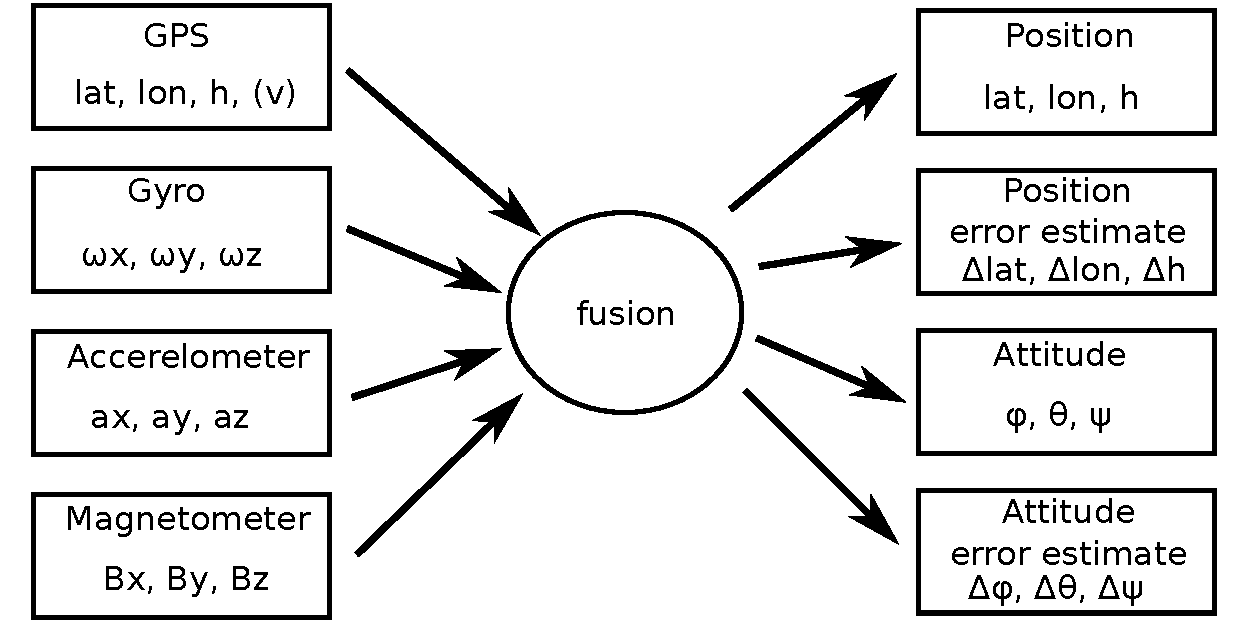
\includegraphics[width=0.8\textwidth]{figures/ADS_diagram.pdf}
\caption{Attitude Determination System overview}
\label{fig:ADS_overview}
\end{figure}

In order to produce high-accuracy attitude estimates and compensate for disadvantages of certain sensor types such as drift and noise, we chose to use a variety of sensors and fuse their information to a combined information.
The facilitated sensors will be (see figure \ref{fig:ADS_overview}):
\begin{itemize}
\item GPS receiver: Provides absolute position values, but has much high-frequency noise
\item Gyroscope: Provides accurate relative pointing direction, but has drift.
\item Accerelometer: Provides absoulte pointing relative to the horizon (gravity) and linear acceleration.
\item Magnetometer: Provides absolute pointing relative to the earth's magnetic field.
\end{itemize}

Combined all together, these sensors provide complete information about the module's attitude.


\subsection{Attitude Determination System Development}

\begin{figure}
\centering
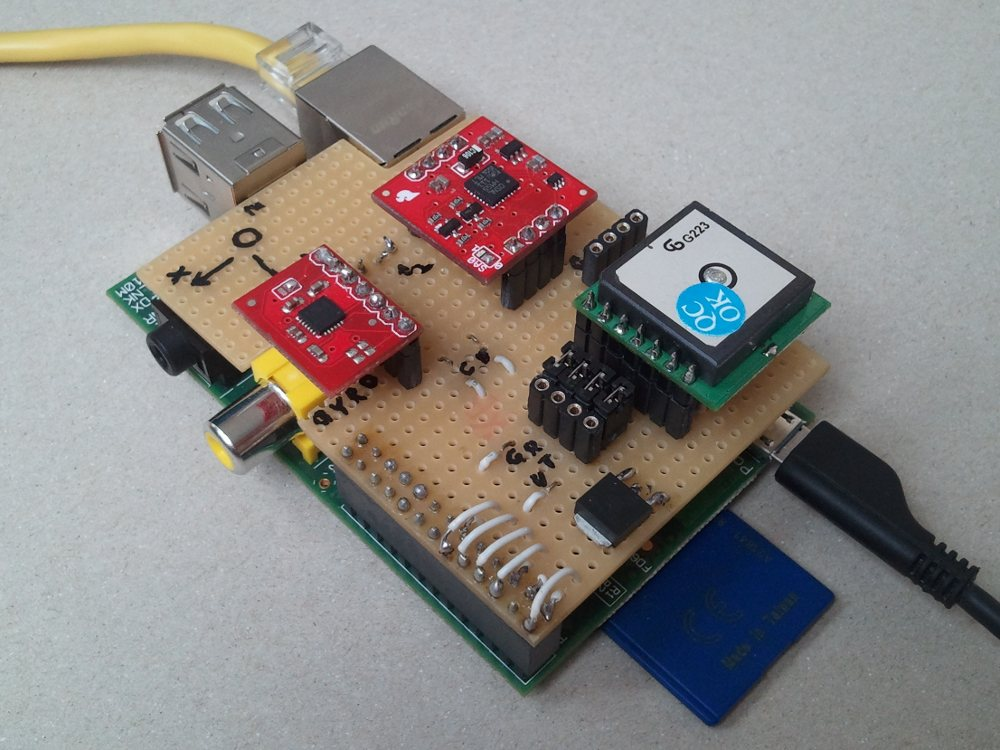
\includegraphics[width=0.8\textwidth]{figures/raspberry-sensors-top.jpg}
\caption{Raspberry Pi computer with our self-constructed sensor shield.
Mounted on the shield are gyroscope (red, left), magnetometer + accelerometer (red, top) and a GPS receiver (green, right).
Also I2C and UART 4-pin sockets are visible as well as a small voltage regulator (bottom) that connects the 3.3V GPS module to the 5V high-current source.}
\label{fig:raspberry-sensors-top}
\end{figure}

\begin{figure}
\centering
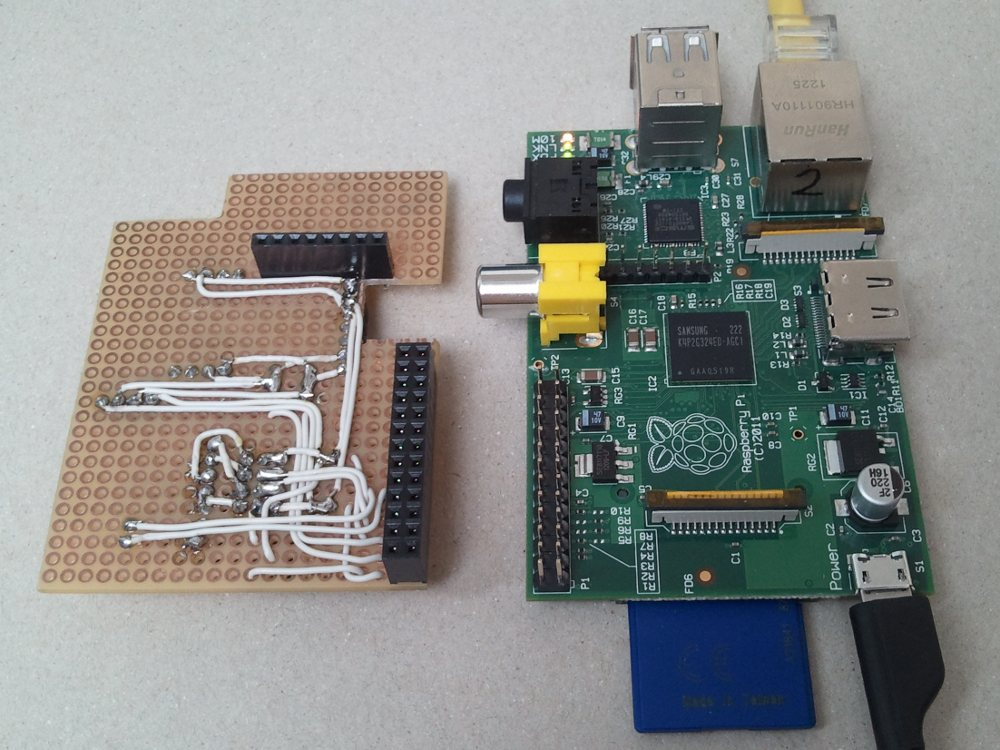
\includegraphics[width=0.8\textwidth]{figures/raspberry-sensors-open.jpg}
\caption{Raspberry Pi computer with our self-constructed plugable sensor shield.
Wiring from the Raspberry Pi 26pin P1 header to individual sensors can be seen on the bottom side of the shield.}
\label{fig:raspberry-sensors-open}
\end{figure}

The attitude determination system was not only developed on the final hardware itself.
For continuation of the development during the semester break a recently released Raspberry Pi minicomputer was privately purchased, which has properties very similar to the Beagle Board and runs a derivate of the Debian operating system.
We created a board to attach a complete set of sensors to the system, which is gyroscope (ITG-3200 from Sparkfun), magnetometer+accelerometer (LSM303 from Sparkfun) and GPS receiver (Venus 6 GPS Module
ST22 from SkyTraq).
All sensors are pluggable and the complete system is shown in \autoref{fig:raspberry-sensors-top}.
The bottom side of the board with wiring cables is shown in \autoref{fig:raspberry-sensors-open}.
This testing system does not yet contain a camera, but it will be added in the future.

In this configuration the whole unit consumes 3W of power and weights 71g (30g for sensors and shield and 41g for the computer).

%% more text until end of august if I [Bastian] find time.


\subsection{Attitude Determination algorithms}
The attitude of the sensing unit could in principle determined by simply integrating the gyro rates up from an initial alignment.
This however will degrade with time because of significant low-frequency drifts, sensor offsets and measurement inaccuracies.

To solve the problem more robust we use a set of 3D gyro-, magnetometer and accelerometer sensors which are fused with our C++ program that runs on the board computer.
Main technique is the Extended Kalman Filter (EKF) which offers and near-optimal estimation with fixed memory usage.
Attitudes are represented as quaternions, which is an elegant and cpu-effective solution.

Offset filtering for the magnetometer and accelerometer is done independently.
We set up an EKF that estimates x- y- and z-offset and total radius along with each new measurement.
%% more text until end of august if I [Bastian] find time.
The measurements are available readily at system startup without calibration, but the accuracy will only improve as soon as measurements from different attitudes are available.
The EKF also accounts for slow offset drifts and similar effects.

Estimation of the gyro offsets and rate scaling is done with combination of acceleration and magnetometer absolute attitude estimations and the gyro-integrated attitude.
This outputs a gyro error value at each measurement step that is used by the Kalman algorithm to estimate the system parameters and calculate a best-estimate attitude.
%% more text until end of august if I [Bastian] find time.

Finally the position is determined independently from the GPS receiver.
This is much simpler than fusing position values from the inertial measurement of the previously described sensors with the absolute GPS position.
With the tight time constraints of the project we choose this simpler method.
However in continuation of the project we want to test the fusion algorithm described in the book ``Stochastic Models -- Estimation and Control'' chapter 6.4.
%% more text until end of august if I [Bastian] find time.


\FloatBarrier
\section{Electrical Circuits}

As compared to the BeagleBone the delivered BeagleBoard's voltage at the pins
of the expansion header is only between 0~V and 1.8~V but the expected voltage
at the supply and the I2C interface for the sensors is 3.3~V additionally to
the external pull-up resistors on the I2C interface also voltage level
converters have to be used.
\\
\\
\textit{More information will be included in the final version...}